% ============================================================
% Question Bank: Modified ch03-01 Integers and Their Opposites (VA SOL Emphasis)
% Topic Title: Integers and Their Opposites — Virginia SOL Emphasis
% VA SOL: 7.1, 7.2 (Rational number comparison, ordering fractions/decimals)
% Questions: 27 (15 MC + 6 SA + 6 Graphical)
% ============================================================

% --- Multiple Choice Questions (15) ---

\begin{practiceQuestion}{m-3-1-q01}{mc}
\begin{questionText}
Which number is the opposite of $-14$?
\end{questionText}
\choiceA{$-14$}
\choiceB{$14$}
\choiceC{$0$}
\choiceD{$\dfrac{1}{14}$}
\correctAnswer{B}
\explanation{The opposite of $-14$ is $14$. Opposites are the same distance from $0$ but on different sides.}
\end{practiceQuestion}

\begin{practiceQuestion}{m-3-1-q02}{mc}
\begin{questionText}
Which inequality correctly compares $-\dfrac{3}{4}$ and $-\dfrac{5}{8}$?
\end{questionText}
\choiceA{$-\dfrac{3}{4} > -\dfrac{5}{8}$}
\choiceB{$-\dfrac{3}{4} < -\dfrac{5}{8}$}
\choiceC{$-\dfrac{3}{4} = -\dfrac{5}{8}$}
\choiceD{$-\dfrac{5}{8} < -\dfrac{3}{4}$}
\correctAnswer{B}
\explanation{Convert: $-\dfrac{3}{4} = -\dfrac{6}{8}$. Since $-\dfrac{6}{8} < -\dfrac{5}{8}$ (farther left on the number line), choice B is correct.}
\end{practiceQuestion}

\begin{practiceQuestion}{m-3-1-q03}{mc}
\begin{questionText}
What is $|{-23}|$?
\end{questionText}
\choiceA{$-23$}
\choiceB{$23$}
\choiceC{$0$}
\choiceD{$\dfrac{1}{23}$}
\correctAnswer{B}
\explanation{Absolute value is the distance from zero: $|{-23}| = 23$.}
\end{practiceQuestion}

\begin{practiceQuestion}{m-3-1-q04}{mc}
\begin{questionText}
Which list is in order from least to greatest?
\end{questionText}
\choiceA{$-0.7,\ -\dfrac{1}{2},\ 0.4,\ \dfrac{3}{5}$}
\choiceB{$\dfrac{3}{5},\ 0.4,\ -\dfrac{1}{2},\ -0.7$}
\choiceC{$-\dfrac{1}{2},\ -0.7,\ 0.4,\ \dfrac{3}{5}$}
\choiceD{$-0.7,\ -\dfrac{1}{2},\ \dfrac{3}{5},\ 0.4$}
\correctAnswer{A}
\explanation{Convert: $-0.7 < -0.5 < 0.4 < 0.6$. Choice A shows the correct order from least to greatest.}
\end{practiceQuestion}

\begin{practiceQuestion}{m-3-1-q05}{mc}
\begin{questionText}
The temperature in Richmond was $-3°$F. In Norfolk it was $-8°$F. Which city was warmer?
\end{questionText}
\choiceA{Norfolk, because $-8$ has a larger digit}
\choiceB{Richmond, because $-3 > -8$}
\choiceC{They are the same temperature}
\choiceD{Norfolk, because $|-8| > |-3|$}
\correctAnswer{B}
\explanation{$-3 > -8$ on the number line. Richmond at $-3°$F is warmer. A larger absolute value means colder for negatives.}
\end{practiceQuestion}

\begin{practiceQuestion}{m-3-1-q06}{mc}
\begin{questionText}
Which rational number is between $-\dfrac{2}{3}$ and $-\dfrac{1}{3}$?
\end{questionText}
\choiceA{$-\dfrac{1}{6}$}
\choiceB{$-\dfrac{5}{6}$}
\choiceC{$-\dfrac{1}{2}$}
\choiceD{$-1$}
\correctAnswer{C}
\explanation{$-\dfrac{2}{3} \approx -0.67$ and $-\dfrac{1}{3} \approx -0.33$. $-\dfrac{1}{2} = -0.5$ lies between them.}
\end{practiceQuestion}

\begin{practiceQuestion}{m-3-1-q07}{mc}
\begin{questionText}
What integer represents the situation: ``A town is $52$ feet below sea level''?
\end{questionText}
\choiceA{$52$}
\choiceB{$-52$}
\choiceC{$0$}
\choiceD{$\dfrac{1}{52}$}
\correctAnswer{B}
\explanation{Below sea level is negative: $-52$ feet.}
\end{practiceQuestion}

\begin{practiceQuestion}{m-3-1-q08}{mc}
\begin{questionText}
Which set of numbers is written in order from greatest to least?
\end{questionText}
\choiceA{$-2.5,\ -1.8,\ -0.3,\ 0.1$}
\choiceB{$0.1,\ -0.3,\ -1.8,\ -2.5$}
\choiceC{$-0.3,\ -2.5,\ 0.1,\ -1.8$}
\choiceD{$0.1,\ -2.5,\ -0.3,\ -1.8$}
\correctAnswer{B}
\explanation{Greatest to least: $0.1 > -0.3 > -1.8 > -2.5$.}
\end{practiceQuestion}

\begin{practiceQuestion}{m-3-1-q09}{mc}
\begin{questionText}
If $|x| = 9$, which values could $x$ be?
\end{questionText}
\choiceA{$9$ only}
\choiceB{$-9$ only}
\choiceC{$9$ or $-9$}
\choiceD{$0$ or $9$}
\correctAnswer{C}
\explanation{$|9| = 9$ and $|{-9}| = 9$. Both are $9$ units from zero.}
\end{practiceQuestion}

\begin{practiceQuestion}{m-3-1-q10}{mc}
\begin{questionText}
Which comparison is true?
\end{questionText}
\choiceA{$-0.45 > -0.4$}
\choiceB{$-\dfrac{7}{10} > -\dfrac{3}{4}$}
\choiceC{$-0.6 > -\dfrac{3}{5}$}
\choiceD{$-\dfrac{1}{3} > -\dfrac{1}{4}$}
\correctAnswer{B}
\explanation{$-\dfrac{7}{10} = -0.70$ and $-\dfrac{3}{4} = -0.75$. Since $-0.70 > -0.75$, choice B is correct. A is false ($-0.45 < -0.4$). C is false (they are equal). D is false ($-0.33 < -0.25$).}
\end{practiceQuestion}

\begin{practiceQuestion}{m-3-1-q11}{mc}
\begin{questionText}
A number and its opposite are $20$ units apart on a number line. What are the two numbers?
\end{questionText}
\choiceA{$5$ and $-5$}
\choiceB{$10$ and $-10$}
\choiceC{$20$ and $-20$}
\choiceD{$0$ and $20$}
\correctAnswer{B}
\explanation{If $x$ and $-x$ are $20$ units apart, then $2x = 20$, so $x = 10$. The numbers are $10$ and $-10$.}
\end{practiceQuestion}

\begin{practiceQuestion}{m-3-1-q12}{mc}
\begin{questionText}
Which decimal is equivalent to $-\dfrac{5}{8}$?
\end{questionText}
\choiceA{$-0.58$}
\choiceB{$-0.625$}
\choiceC{$-0.65$}
\choiceD{$-0.585$}
\correctAnswer{B}
\explanation{$5 \div 8 = 0.625$. With the negative: $-\dfrac{5}{8} = -0.625$.}
\end{practiceQuestion}

\begin{practiceQuestion}{m-3-1-q13}{mc}
\begin{questionText}
A parking garage has floors labeled $-3, -2, -1, 0, 1, 2$. A car on floor $-2$ goes up $4$ floors. What floor is the car on?
\end{questionText}
\choiceA{$-6$}
\choiceB{$2$}
\choiceC{$-2$}
\choiceD{$6$}
\correctAnswer{B}
\explanation{$-2 + 4 = 2$. The car is on floor $2$.}
\end{practiceQuestion}

\begin{practiceQuestion}{m-3-1-q14}{mc}
\begin{questionText}
Which fraction is closest to $0$ on a number line?
\end{questionText}
\choiceA{$-\dfrac{7}{8}$}
\choiceB{$\dfrac{2}{3}$}
\choiceC{$-\dfrac{1}{5}$}
\choiceD{$\dfrac{3}{4}$}
\correctAnswer{C}
\explanation{Absolute values: $\dfrac{7}{8} = 0.875$, $\dfrac{2}{3} \approx 0.667$, $\dfrac{1}{5} = 0.2$, $\dfrac{3}{4} = 0.75$. $\dfrac{1}{5}$ is smallest, so $-\dfrac{1}{5}$ is closest to $0$.}
\end{practiceQuestion}

\begin{practiceQuestion}{m-3-1-q15}{mc}
\begin{questionText}
The opposite of the opposite of $-7$ is:
\end{questionText}
\choiceA{$7$}
\choiceB{$-7$}
\choiceC{$0$}
\choiceD{$14$}
\correctAnswer{B}
\explanation{Opposite of $-7$ is $7$. Opposite of $7$ is $-7$. The opposite of the opposite returns to the original number.}
\end{practiceQuestion}

% --- Short Answer Questions (6) ---

\begin{practiceQuestion}{m-3-1-q16}{sa}
\begin{questionText}
Order from least to greatest: $-\dfrac{3}{5},\ 0.2,\ -0.75,\ \dfrac{1}{4}$.
\end{questionText}
\correctAnswer{$-0.75,\ -\dfrac{3}{5},\ 0.2,\ \dfrac{1}{4}$}
\explanation{Convert: $-0.75,\ -0.6,\ 0.2,\ 0.25$. Order: $-0.75 < -0.6 < 0.2 < 0.25$.}
\end{practiceQuestion}

\begin{practiceQuestion}{m-3-1-q17}{sa}
\begin{questionText}
What integer is represented by ``a gain of $\$250$''?
\end{questionText}
\correctAnswer{$+250$ or $250$}
\explanation{A gain is positive: $+250$ or $250$.}
\end{practiceQuestion}

\begin{practiceQuestion}{m-3-1-q18}{sa}
\begin{questionText}
Find the distance between $-3.8$ and $2.7$ on a number line.
\end{questionText}
\correctAnswer{$6.5$ units}
\explanation{Distance $= |{-3.8} - 2.7| = |{-6.5}| = 6.5$ units.}
\end{practiceQuestion}

\begin{practiceQuestion}{m-3-1-q19}{sa}
\begin{questionText}
If $a = -\dfrac{3}{4}$ and $b = \dfrac{5}{8}$, compare $a$ and $b$ using $<$, $>$, or $=$.
\end{questionText}
\correctAnswer{$a < b$ (or $-\dfrac{3}{4} < \dfrac{5}{8}$)}
\explanation{$-\dfrac{3}{4} = -0.75$ and $\dfrac{5}{8} = 0.625$. Since $-0.75 < 0.625$, $a < b$.}
\end{practiceQuestion}

\begin{practiceQuestion}{m-3-1-q20}{sa}
\begin{questionText}
The elevations of two locations are $-18$ feet and $-45$ feet. Which is higher?
\end{questionText}
\correctAnswer{$-18$ feet}
\explanation{$-18 > -45$ on the number line, so $-18$ feet is the higher elevation.}
\end{practiceQuestion}

\begin{practiceQuestion}{m-3-1-q21}{sa}
\begin{questionText}
What is $|{-15.3}| - |{-8.7}|$?
\end{questionText}
\correctAnswer{$6.6$}
\explanation{$|{-15.3}| = 15.3$ and $|{-8.7}| = 8.7$. Difference: $15.3 - 8.7 = 6.6$.}
\end{practiceQuestion}

% --- Graphical Questions (3 GMC + 3 GSA) ---

\begin{practiceQuestion}{m-3-1-q22}{gmc}
\begin{questionText}
The number line shows points $P$, $Q$, $R$, and $S$. Which point represents $-\dfrac{3}{4}$?

\begin{center}
\begin{tikzpicture}
  \draw[thick,->] (-2.5,0) -- (2.5,0);
  \foreach \x in {-2,-1,0,1,2} \draw (\x,0.1) -- (\x,-0.1) node[below,font=\small] {$\x$};
  \foreach \x in {-1.5,-0.5,0.5,1.5} \draw (\x,0.05) -- (\x,-0.05);
  \fill[funBlue] (-1.5,0) circle (0.1) node[above=4pt,font=\small] {$P$};
  \fill[funRed] (-0.75,0) circle (0.1) node[above=4pt,font=\small] {$Q$};
  \fill[funGreen] (0.25,0) circle (0.1) node[above=4pt,font=\small] {$R$};
  \fill[funOrange] (1.25,0) circle (0.1) node[above=4pt,font=\small] {$S$};
\end{tikzpicture}
\end{center}
\end{questionText}
\choiceA{$P$}
\choiceB{$Q$}
\choiceC{$R$}
\choiceD{$S$}
\correctAnswer{B}
\explanation{$-\dfrac{3}{4} = -0.75$, which is halfway between $-1$ and $-\dfrac{1}{2}$. Point $Q$ is at $-0.75$.}
\end{practiceQuestion}

\begin{practiceQuestion}{m-3-1-q23}{gmc}
\begin{questionText}
The table shows daily low temperatures in a Virginia city during one week. Which day had the absolute value that was greatest?

\begin{center}
\begin{tabular}{|l|c|}
\hline
\textbf{Day} & \textbf{Low Temp (°F)} \\
\hline
Monday & $4$ \\ \hline
Tuesday & $-7$ \\ \hline
Wednesday & $-2$ \\ \hline
Thursday & $6$ \\ \hline
Friday & $-9$ \\ \hline
\end{tabular}
\end{center}
\end{questionText}
\choiceA{Monday}
\choiceB{Tuesday}
\choiceC{Thursday}
\choiceD{Friday}
\correctAnswer{D}
\explanation{Absolute values: $4, 7, 2, 6, 9$. Friday's $|{-9}| = 9$ is the greatest absolute value.}
\end{practiceQuestion}

\begin{practiceQuestion}{m-3-1-q24}{gmc}
\begin{questionText}
A vertical thermometer shows $-5°$C. Which temperature is $8$ degrees warmer?

\begin{center}
\begin{tikzpicture}[scale=0.5]
  \draw[thick] (0,-7) -- (0,7);
  \foreach \y in {-6,...,6} \draw (-0.2,\y) -- (0.2,\y) node[right,font=\small] {$\y$};
  \fill[red!40] (-0.15,-7) rectangle (0.15,-5);
  \draw[thick,<->,funGreen] (0.6,-5) -- (0.6,3) node[midway,right,font=\small] {$+8°$};
\end{tikzpicture}
\end{center}
\end{questionText}
\choiceA{$-13°$C}
\choiceB{$-3°$C}
\choiceC{$3°$C}
\choiceD{$13°$C}
\correctAnswer{C}
\explanation{$-5 + 8 = 3°$C.}
\end{practiceQuestion}

\begin{practiceQuestion}{m-3-1-q25}{gsa}
\begin{questionText}
Plot the following rational numbers on the number line and list them from least to greatest: $\dfrac{1}{2},\ -1.5,\ -\dfrac{1}{4},\ 0.75$.

\begin{center}
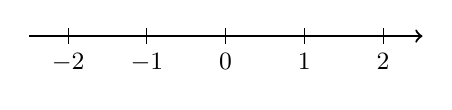
\begin{tikzpicture}
  \draw[thick,->] (-2.5,0) -- (2.5,0);
  \foreach \x in {-2,-1,0,1,2} \draw (\x,0.1) -- (\x,-0.1) node[below,font=\small] {$\x$};
\end{tikzpicture}
\end{center}
\end{questionText}
\correctAnswer{$-1.5,\ -\dfrac{1}{4},\ \dfrac{1}{2},\ 0.75$}
\explanation{Convert: $-1.5,\ -0.25,\ 0.5,\ 0.75$. Order: $-1.5 < -0.25 < 0.5 < 0.75$.}
\end{practiceQuestion}

\begin{practiceQuestion}{m-3-1-q26}{gsa}
\begin{questionText}
The table shows elevations of Virginia landmarks. What is the difference in elevation between the highest and lowest?

\begin{center}
\begin{tabular}{|l|c|}
\hline
\textbf{Location} & \textbf{Elevation (ft)} \\
\hline
Mt. Rogers & $5{,}729$ \\ \hline
Chesapeake Bay shore & $0$ \\ \hline
Back Bay (tidal) & $-2$ \\ \hline
\end{tabular}
\end{center}
\end{questionText}
\correctAnswer{$5{,}731$ feet}
\explanation{$5{,}729 - (-2) = 5{,}729 + 2 = 5{,}731$ feet difference.}
\end{practiceQuestion}

\begin{practiceQuestion}{m-3-1-q27}{gsa}
\begin{questionText}
A number line shows the boiling points (°C) of three substances. What is the distance between the lowest and highest boiling points?

\begin{center}
\begin{tikzpicture}[scale=0.03]
  \draw[thick,->] (-210,0) -- (120,0);
  \draw (-196,2) -- (-196,-2) node[below,font=\small] {$-196$};
  \draw (0,2) -- (0,-2) node[below,font=\small] {$0$};
  \draw (100,2) -- (100,-2) node[below,font=\small] {$100$};
  \fill[funBlue] (-196,0) circle (3) node[above=6pt,font=\small] {Nitrogen};
  \fill[funGreen] (0,0) circle (3) node[above=6pt,font=\small] {Water freezes};
  \fill[funRed] (100,0) circle (3) node[above=6pt,font=\small] {Water boils};
\end{tikzpicture}
\end{center}
\end{questionText}
\correctAnswer{$296°$C}
\explanation{Distance $= |100 - (-196)| = |100 + 196| = 296°$C.}
\end{practiceQuestion}
